%----------------------------------------------------------------------------
\chapter{Javaslat további funkciókra}\label{chapter:features}
%----------------------------------------------------------------------------
Diplomaterv feladatkiírásom része, hogy tegyek javaslatot olyan új modulokra vagy módosításokra, melyekkel a Jporta funkcionalitása bővíthető lenne.
A portál fejlesztése közben sok hasznos ötlet látott napvilágot.
Ebben a fejezetben az általam leghasznosabbnak ítélt két funkció indokoltságáról fogok beszélni, illetve vázolom egy lehetséges megvalósításhoz szükséges tervezési és implementációs lépéseket.

\section{Csapatrendszer}
Az első javaslatom egy csapatmunka támogatását lehetővé tevő funkció Jportába történő integrálása lenne.
A csapatrendszer feladata, hogy lehetővé tegye hallgatói csapatok kialakítását mind hallgatók, mind oktatók által, illetve a Jporta meglévő adminisztrációs funkcióit (értékelés, jelenlét, stb.) kiterjessze egyéni hallgatókról csapatokra.

A Jporta fejlesztésének megkezdésekor felmerült IIT-n használt egyéb, hasonló célú, oktatási rendszerek konszolidációja az új portálba, amivel a sok különböző alkalmazás működtetésére, karbantartására szánt idő és erőforrások csökkenthetőek lennének.
Az egyik ilyen rendszer a Hercules, melynek többek között a Szoftver projekt laboratórium -- régi nevén Szoftver labor 4. -- tárgy oktatásában van szerepe.
A tárgy keretében a hallgatók csapatban végzik el egy kisebb komplexitású szoftver tervezését, fejlesztését és dokumentálását.
A Hercules egyik legfontosabb funkciója is ehhez kapcsolódik, mégpedig hogy a félév elején biztosítja a hallgatók számára az említett csapatok kialakítását.
A jelenlegi rendszerben a hallgatóknak egy hét áll rendelkezésére a félév elején, hogy önállóan kialakítsák az 5-6 főből álló csapatokat, melyeket a Hercules felületén regisztrál a csapat vezetője.
A csapat regisztrációjakor meg kell adnia a csapat egyedi nevét, a csapattagok pedig a Neptun kódjukkal kerülnek azonosításra.
A határidő letelte után csapat nélkül maradt hallgatókat a tárgy felelőse osztja be csapatokba saját belátása szerint. 

\subsection{Tervezés}
A tervezés első lépése a Hercules fent leírt funkciójának megismerése és az új rendszerhez való illesztési lehetőségeinek vizsgálata.
Ezután következhet csak egy új, csapatokat modellező osztály és a hozzá kapcsolódó üzleti logika megvalósítását segítő segédosztályok definiálása, továbbá a már meglévő kódrészek hozzáigazítása az új fejlesztéshez.

A csapatrendszer egyik alapvető funkciója a csapatok kialakítása.
A Hercules által implementált metódus kissé körülményes, kevés rugalmasságot biztosít a felhasználók számára.
Ezért az új rendszerben ennek a funkciónak némi átalakítással, modernizálással kell megvalósulni, igazodva a Jporta adottságaihoz, és kihasználva azokat.

A csapatalakítás menete az új rendszerben lehetne a következő:
\begin{enumerate}
    \item A hallgató belép a portálra és kiválasztja a tárgyat, amelyhez csapatot kíván alakítani.
    \item Kiválasztja az \textit{Új csapat alakítása} funkciót és megadja a csapat nevét.
    \item A létrejött csapatba meginvitálja hallgatótársait, amiről azok értesítést kapnak a Jporta beépített üzenetküldő rendszerén keresztül.
    \item A csapat meghívott tagjai eldöntik, hogy elfogadják-e a meghívást.
\end{enumerate}
Ebben az elgondolásban a csapatot létrehozó hallgató tölti be a csapatkapitány szerepét, ezért neki -- a csapatalakítás időszakában -- lehetősége van a csapatból csapattagok eltávolítására, illetve új csapattagok meghívására.
A csapatkapitány mindenképp részét képezi a csapatnak.
Minden hallgató tárgyanként legfeljebb egy csapatnak lehet tagja.
Azok a hallgatók, akik már tagjai egy csapatnak, de nem kapitányai csapatuknak, megszüntethetik tagságukat, és ezután van lehetőségük új csapatba invitációt elfogadni, vagy saját csapatot létrehozni.

A tárgy adatlapján az oktató megadhatja, hogy a tárgyban csapatmunka támogatására van-e szükség, és ha igen, akkor milyen alsó és felső korlát van a csapatok méretére, illetve mely időtartományban van lehetősége a hallgatóknak csapatot alakítani.
A tárgy oktatóinak bármikor lehetősége van új csapat létrehozására, illetve a meglévő csapatok törlésére, módosítására, de fontos, hogy ezzel a jogosultságukkal csak indokolt esetben éljenek.
Különös figyelmet kell fordítani a hallgatók csapatok közti mozgatására, mivel ez egy igen gyakori művelet, ami kitüntetett támogatás nélkül nehézkes és időigényes feladattá tud válni.

A csapatrendszer bevezetése miatt a portál megjelenésének és kezelésének is változnia kell.
Az oktatók egy tárgy adatlapján eddig az egyes hallgatókat értékelhették, adminisztrálhatták az órákon való részvételüket, adhattak ki nekik feladatot.
Az új rendszerben viszont, a csapatmunkát igénylő tárgyaknál ezeknek a funkcióknak csapatokon kell elvégezhetőeknek lenniük.

\subsection{Megvalósítás}
A csapatrendszer implementálásának alapja a csapatot megtestesítő Django modell létrehozása.
Ez az osztály írja le, milyen attribútumok tárolódnak az egyes csapatokról az adatbázisban, illetve hogy a Jporta rendszerének többi entitásával milyen kapcsolatban áll (lásd \ref{figure:teams-after}. ábra).
Ugyanez az osztály implementálja a csapatokhoz szorosan kapcsolódó üzleti logikát is.
Ahogy az a \ref{figure:teams-before}. és \ref{figure:teams-after}. ábra összehasonlításából jól látszik, a változtatások után a felhasználót reprezentáló \texttt{SwdUser} osztályt sok esetben a \texttt{Team} osztály váltja fel, ugyanakkor a tervezésnél már említettem, hogy a csapatok használata tárgyanként eltérő lehet, egy kapcsolótól függ csupán, melyet a tárgy oktatója választ meg.
Ezt a kettősséget úgy oldanám fel, hogy a háttérben mindkét esetben csapatokkal dolgozik a modell, ám ha az adott tárgy nem igényel csapatmunka-támogatást, akkor a rendszer minden felhasználó számára automatikusan létrehozza a felhasználó egyszemélyes csapatát.
A felhasználók számára ez egy teljesen transzparens folyamat, a megjelenítés a tárgyhoz beállítása alapján dönti el, hogy csapatok vagy egyéni felhasználók megjelenítésére van-e szükség egy adott esetben.

\begin{figure}[h]
    \centering
    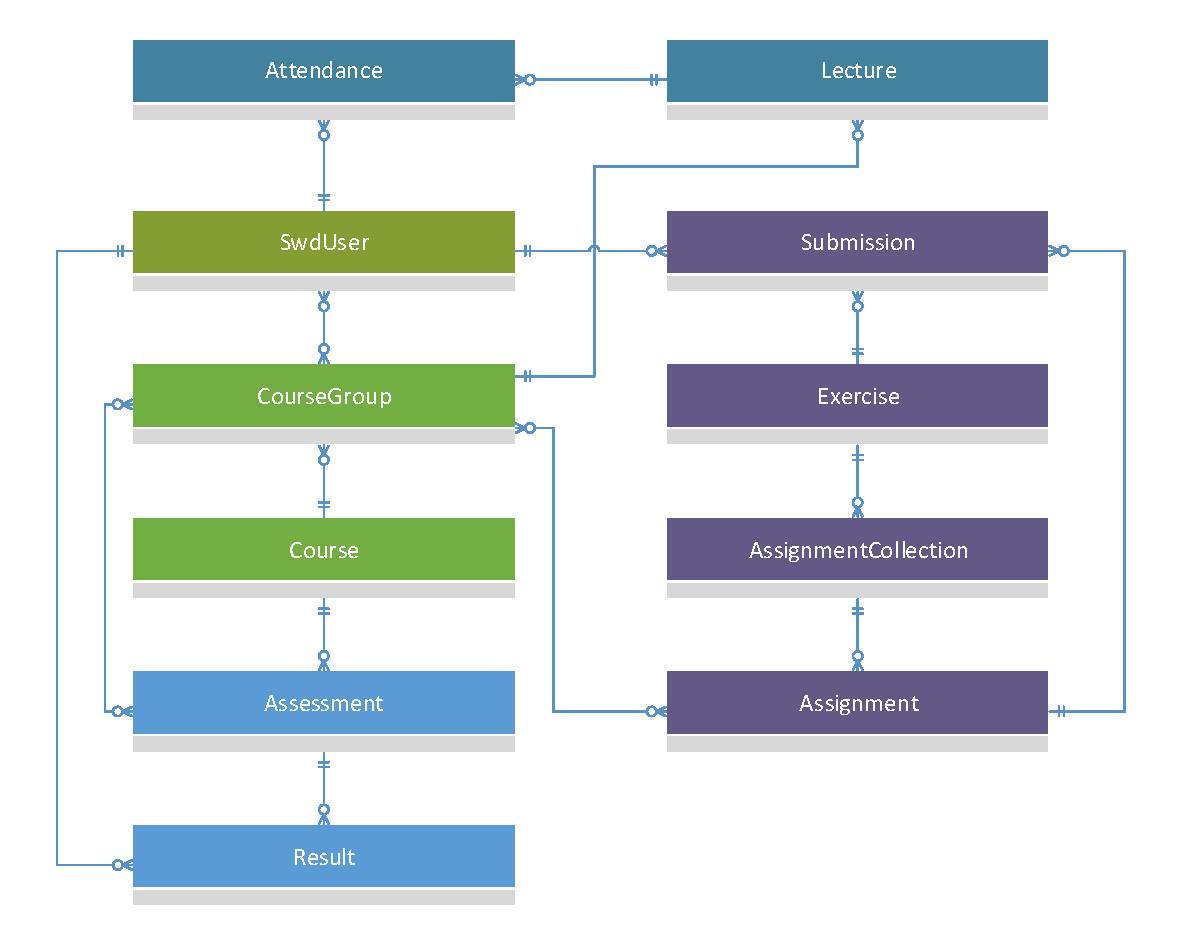
\includegraphics[width=\textwidth]{figures/teams-before}
    \caption{Jporta modellje csapatok nélkül}
    \label{figure:teams-before}
\end{figure}

\begin{figure}[h]
    \centering
    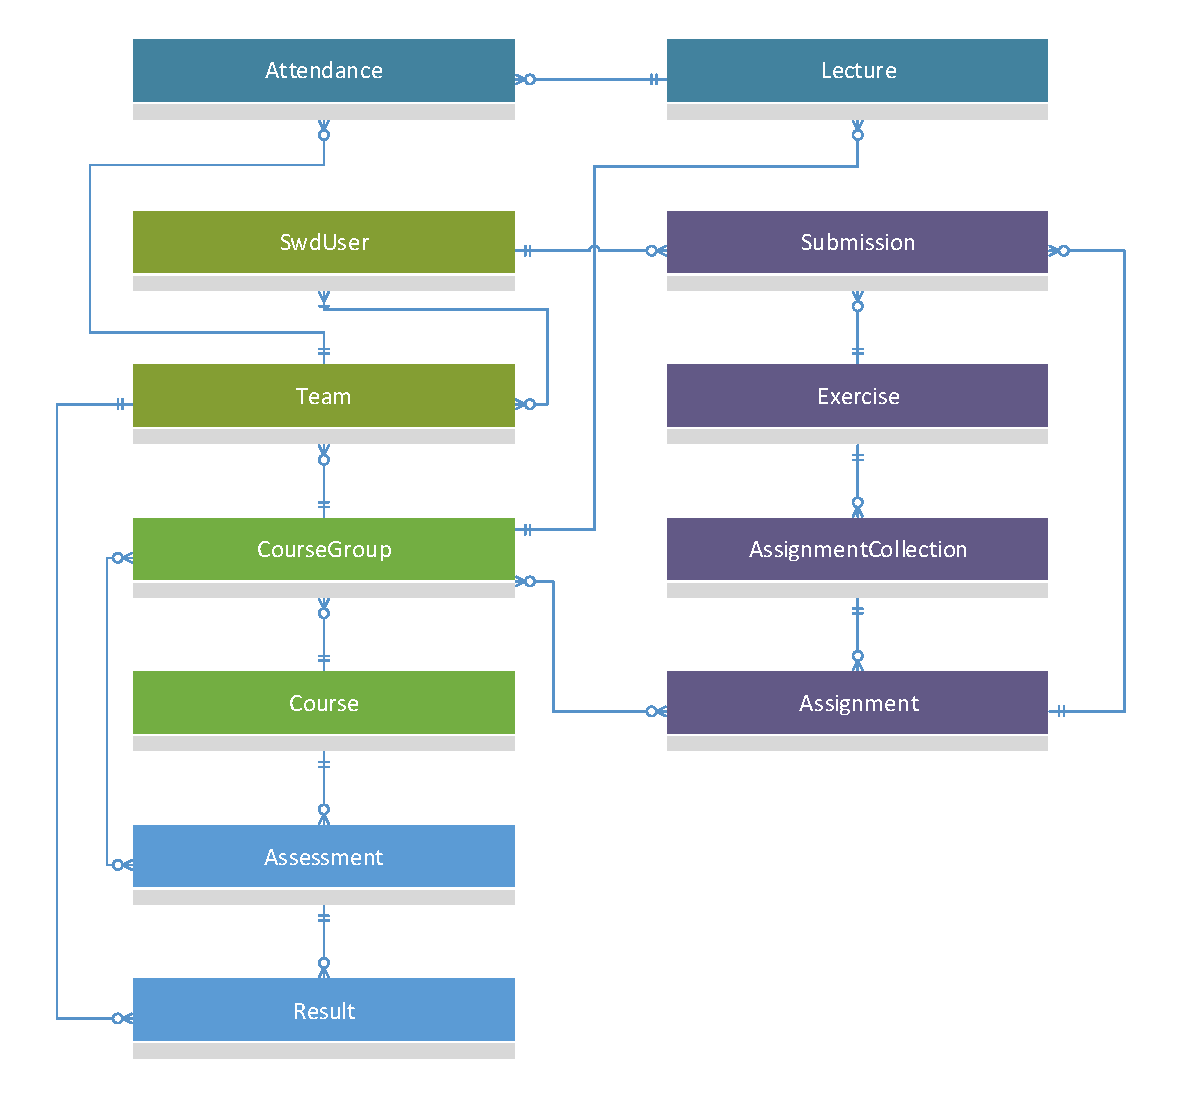
\includegraphics[width=\textwidth]{figures/teams-after}
    \caption{Jporta modellje csapatokkal}
    \label{figure:teams-after}
\end{figure}

További változás, hogy az eddig a kurzuscsoportok tagjainak nyilvántartására használt, Djangoba beépítetten érkező \texttt{Group} osztályt a fejlesztés során ki kell váltani egy több-több kapcsolatot nyilvántartó ``kapcsolótáblával'', mivel az egyes kurzuscsoportok (\texttt{CourseGroup}) most már nem felhasználóhoz (\texttt{SwdUser}), hanem csapatokhoz (\texttt{Team}) kapcsolódnak, ezeknek a tárolását viszont a \texttt{Group} osztály nem támogatja.

\section{Integráció verziókövető rendszerrel}
A második javaslatom egy olyan funkció beépítésére vonatkozik, amely lehetővé tenné, hogy a hallgatók egy verziókezelő szoftver segítségével tudják beadni megoldásaikat.
Ezzel a hallgatók a verziókövető rendszerek használatát a szoftverfejlesztéssel egybekötve sajátíthatnák el, ami egyrészt jó habitus, másrészt követi a valódi fejlesztés menetét.

A verziókezelő rendszerek alapvető megértése és használatuk elsajátítása szinte minden szoftverfejlesztő számára nélkülözhetetlen.
A általunk létrehozott állományok különböző állapotainak tárolása több előnnyel is jár.
Például könnyedén megtudhatjuk, mi változott a legutóbbi állapot óta, vagy akár két régebbi állapot között.
Ezt a tudást felhasználhatjuk akár egyfajta munkanaplóként is, vagy bármikor könnyedén visszaállíthatunk felülírt vagy törölt részeket.

\subsection{Tervezés}
Az első lépés egy megfelelő verziókövető rendszer kiválasztása, majd eztután következhet az integráció részleteinek tervezése.

A változáskövető rendszerek manapság két nagy csoportra oszthatók: \textit{központi} (\textit{centralized}, pl. CVS, SVN, TFS) és \textit{elosztott} (\textit{distributed}, pl. Bazaar, Git, Mercurial).
Kezdetben a fejlesztők központi verziókezelő rendszereket készítettek és használtak, mivel így volt a legegyszerűbb a tartalmak megosztása, ezáltal a közös munka.
Az utóbbi 10 év során azonban az elosztott rendszerek fokozatosan, de egyértelműen átvették a vezetést, köszönhetően a könnyen hozzáférhető interneteléréseknek, és a nyílt forráskódú szoftvereknél gyakori közösségi fejlesztés elterjedésének, melynek magasfokú párhuzamosság-igényével a központi rendszerek nem tudnak megbirkózni.
A központi verziókövetők legnagyobb hátránya az elosztottakkal szemben, hogy utóbbiak képesek szimulálni az előbbiek egy szerver--több kliens konfigurációját, de emellett sokkal nagyobb rugalmasságot és több funkciót biztosítanak.
Ezen okok miatt én egy elosztott verziókezelő rendszert, a Gitet választanám.

A Gitet 2005-ben Linus Torvalds készítette a Linux kernel fejlesztéséhez, de azóta napjaink egyik legelterjedtebb megoldásává vált.
A Git alapvető használata a parancssorból sem túlzottan bonyolult -- köszönhetően egyszerű felépítésének --, de létezik sok grafikus alkalmazás is\footnote{Egy átfogó listáért lásd: \url{https://git.wiki.kernel.org/index.php/Interfaces,\_frontends,\_and\_tools\#Graphical\_Interfaces}}, melyekkel kezdők és profik egyaránt könnyedén elboldogulnak, sőt, minden elterjedtebb integrált fejlesztőkörnyezet tartalmaz Gitet támogató beépülő modulokat.
A Git emellett gyors, biztonságos, és a legtöbb operációs rendszeren támogatott.

Ahogy más elosztott verziókezelő rendszerekben, a Gitben is különválik a \textit{commitolás} -- a fájlok pillanatnyi állapotának rögzítése --, és a \textit{pusholás} -- a létrejött commitok publikálása, megosztása -- művelete.
A fejlesztő egy feladat megoldása közben tetszőleges számú commitot készíthet, ám ezekről mások csak akkor értesülnek, amikor a fejlesztő egy távoli tárolóval szinkronizál, megosztja a változásait: pushol.

A portálnak tehát biztosítania kell egy verziókezelt tárolót a hallgató számára, amelybe feltöltheti megoldásait a változáskövető rendszer segítségével.
Amikor a hallgató ebbe a tárolóba feltölti legújabb megoldását, a Jportában keletkeznie kell egy beadásnak a fájlok legfrissebb állapotát felhasználva.

Mivel a Jportát több hallgató is használja, továbbá egy hallgató több feladatra is küld be megoldásokat, felmerülhet a kérdés, hogy hány tárolóra van ekkor szükség összesen?
A Git képes egy tárolón belül több különböző fejlesztési ág -- \textit{branch} -- párhuzamos menedzselésére is.
Ezt felhasználva akár egyetlen tároló is elegendő lenne, ha minden felhasználó--feladatkiadás páros számára külön ágat hozunk létre.
Ennek a rendszernek a használata azonban körülményes és ellenkezik a megszokott használati mintákkal is.
Az egy tárolós megoldás és a másik véglet -- vagyis hogy minden felhasználó minden feladatához külön tárolót biztosítunk -- között több változat is elképzelhető, ám véleményem szerint ez utóbbi a legelőnyösebb választás, mégpedig azért, mert így a hallgatók egy majdnem teljes értékű verziótároló szolgáltatást vehetnek igénybe a portálon.

Néhány megkötést azonban mégis tenni kell a tároló használatával kapcsolatban.
Az egyik megkötés, hogy a beadórendszer csak egy kitüntetett -- pl. \textit{master} -- ág módosításait figyeli, így a hallgató a valódi fejlesztéseknél is alkalmazott sémát követhet a verziókövető használatakor.
A másik megkötés, hogy ezen az ágon nem engedélyezett az úgynevezett \textit{forced push} művelet, vagyis az ág történelmének felülírása, mivel ez inkonzisztens állapotba hozhatná a portált -- pl. eltűnhet olyan állapot, amiből beadás készült.

A Git több protokollt is támogat a tárolók közötti kommunikációra.
Ezek közül nekünk olyanra van szükségünk, amely támogatja a felhasználók azonosítását, mert csak így érhetjük el, hogy kizárólag a Jporta felhasználói érhessék el a tárolókat, illetve minden felhasználó csak a saját tárolóihoz férjen hozzá.
A két szóbajövő protokoll a HTTPS és az SSH.
Mindkét protokoll biztonságos és ajánlott, különösebb hátránnyal egyik sem rendelkezik.
A legnagyobb eltérés a kettő között az azonosítás módjában rejlik.
Míg a HTTPS protokoll használatakor a HTTP-nél megszokott azonosítási módszerek legtöbbje alkalmazható (pl. felhasználónév--jelszó páros), addig SSH fölött kizárólag SSH kulcspárral azonosíthatja magát a felhasználó.
\cite{ProGit}

A Git működéséről és használatáról bővebb információkat \cite{ProGit} ad. 

\subsection{Megvalósítás}
Az integráció megvalósításához egy kapcsolat létrehozására van szükség a verziókövető és a Jporta között.
A verziókövetőnek tudnia kell jelezni a portálnak, amikor új beadás történt, a portálnak pedig hozzá kell tudnia férni a verziókezelő által tárolt adatokhoz.

A kapcsolat első irányát, vagyis az új verziók érkezésének jelzését, a Git \textit{hook} funkciójával lehetne megvalósítani.
A hookok olyan programok, amelyeket a Git valamilyen esemény hatására automatikusan lefuttat.
Az egyik ilyen hook a \textit{post-update hook}, amelyet a \textit{git-reveive-pack} hív meg a -- küldő szempontjából -- távoli tárolón, miután a frissítés befejeződött.
Ezt a működést a helyi gépen kiadott \texttt{git push} parancs idézi elő, vagyis pontosan akkor történik, mikor a felhasználó szinkronizálni szeretné változásait a Jportával.
\cite{GitHooks}
A Jporta esetében a hook által végrehajtott program lehetne egy egyszerű -- például Python nyelvű -- szkript, ami a webportálon beadott megoldások regisztrációjával analóg műveletet hajt végre.
A programot a Git tároló gyökerében található \texttt{hooks} könyvtárban kell elhelyezni \texttt{post-update} névvel.  % `git rev-parse --git-dir`/hooks/post-update vagy `git config core.hooksPath`/post-update, ha felül van írva
Ezenkívül az állománynak futtathatónak kell lennie a Git műveleteket végző felhasználó által.

Ahhoz, hogy a portál ezután hozzá tudjon férni a verziókövetőben tárolt adatokhoz, a pygit2 függvénykönyvtár használatát javasolnám.
Ez a függvénykönyvtár a libgit2 megosztott könyvtárhoz biztosít hozzáférést Python nyelvből, így a fontosabb Git műveletek elvégezhetőek segítségével. \cite{pygit2}

A hallgatók és a Jportán lévő verziókezelt tárolók összekapcsolását az előző szakaszban ismertetett protokollokon keresztül valósítanám meg.
Mielőtt viszont a hallgató publikálhatná megoldásait a portálra, szükség van a verziókezelt tárolók létrehozására az adott felhasználó--feladatkiadás páros számára.
A tárolók automatikus létrehozása feleslegesen terhelheti a portál erőforrásait, hiszen nem biztos, hogy minden hallgató minden feladatához használni fogja ezt a lehetőséget, ezért jobb megoldás lehet, ha a hallgatóknak a webportálon maguknak kell indítványozniuk a tároló létrehozását minden feladatkiadás esetén.
Ez a felfogás összhangban van a legtöbb verziókövető, illetve más verziótároló szolgáltatást nyújtó portálok -- pl. BitBucket, GitHub -- működésével is.